\documentclass[conference]{IEEEtran}
\IEEEoverridecommandlockouts
\usepackage{iftex}
\usepackage{cite}
\usepackage{amsmath}
\ifXeTeX
  \usepackage{newtxmath}
  \usepackage[no-math]{fontspec}
  \setmainfont{texgyretermes}[Extension=.otf, UprightFont=*-regular, BoldFont=*-bold,
    ItalicFont=*-italic, BoldItalicFont=*-bolditalic, Language=Turkish,
    % küçük büyük harfler Türkçe i'yi noktasız I yapıyor; başlıklarda kalın yazı kullanılır
    SmallCapsFont=texgyretermes-bold, SmallCapsFeatures={Extension=.otf}]
\else
  \usepackage[T1]{fontenc}
  \usepackage[utf8]{inputenc}
  \usepackage{newtxtext,newtxmath}
\fi
\usepackage[turkish,shorthands=off]{babel}
\usepackage{graphicx}
\usepackage{booktabs}
\usepackage{multirow}
\usepackage{array}
\usepackage{tabularx}
\usepackage{longtable}
\usepackage{xcolor}
\usepackage{tikz}
\usetikzlibrary{positioning,arrows.meta,fit,backgrounds}
\usepackage[hidelinks]{hyperref}
\usepackage{url}
\renewcommand{\IEEEkeywordsname}{Anahtar Kelimeler}

% ---- Teslim bilgileri: yalnızca bu üç satır düzenlenir --------------------
\newcommand{\VideoURL}{\url{https://youtu.be/VIDEO-LINK-HERE}}
\newcommand{\RepoURL}{\url{https://github.com/mrayenesay/leukemia-all-aml-ml}}
\newcommand{\Affil}{Yapay Zeka Programı, Fen Bilimleri Enstitüsü\\
Eskişehir Osmangazi Üniversitesi, Eskişehir, Türkiye}
% ---------------------------------------------------------------------------

% AUTO-GENERATED by scripts/make_report_assets.py -- do not edit
\newcommand{\GolubN}{72}
\newcommand{\GolubP}{7{,}129}
\newcommand{\GolubMapped}{6{,}434}
\newcommand{\GolubTrainALL}{27}
\newcommand{\GolubTrainAML}{11}
\newcommand{\GolubTestALL}{20}
\newcommand{\GolubTestAML}{14}
\newcommand{\GolubValues}{513{,}288}
\newcommand{\GolubNonFinite}{0}
\newcommand{\GolubNegPct}{28.7}
\newcommand{\GolubBelowPct}{32.7}
\newcommand{\GolubAbovePct}{0.83}
\newcommand{\GolubMin}{-28{,}400}
\newcommand{\GolubMax}{71{,}369}
\newcommand{\GolubAffx}{58}
\newcommand{\GolubAllNeg}{233}
\newcommand{\GolubCallP}{28.2}
\newcommand{\GolubCallA}{70.2}
\newcommand{\GolubCallM}{1.6}
\newcommand{\GolubMedP}{662}
\newcommand{\GolubMedA}{33}
\newcommand{\GolubNeverPresent}{1{,}971}
\newcommand{\GolubPresMin}{19.1}
\newcommand{\GolubPresMax}{40.5}
\newcommand{\GolubFilt}{3{,}859}
\newcommand{\GolubSkewRaw}{7.08}
\newcommand{\GolubSkewLog}{0.55}
\newcommand{\GolubRhoLin}{0.95}
\newcommand{\GolubRhoLog}{0.18}
\newcommand{\GolubPCOne}{10.8}
\newcommand{\GolubPCTwo}{8.8}
\newcommand{\GolubCumTen}{49.6}
\newcommand{\GolubNEighty}{37}
\newcommand{\GolubPCOneAUC}{0.984}
\newcommand{\GolubSilPCA}{0.17}
\newcommand{\GolubSilTSNE}{0.40}
\newcommand{\GolubSig}{945}
\newcommand{\GolubSigOne}{567}
\newcommand{\GolubSigMWU}{1{,}014}
\newcommand{\GolubUpAML}{462}
\newcommand{\GolubUpALL}{483}
\newcommand{\GolubRhoSNR}{0.999}
\newcommand{\GolubARI}{0.94}
\newcommand{\GolubTop}{MGST1, CST3, TCF3, ZYX, CD33, APLP2, CD79B, POU2AF1, DNTT, CCND3}
\newcommand{\GolubPresTrain}{29.0}
\newcommand{\GolubPresTest}{27.3}
\newcommand{\GolubPresP}{0.071}
\newcommand{\GolubQP}{0.016}
\newcommand{\GolubQTrain}{482}
\newcommand{\GolubQTest}{421}
\newcommand{\GolubKSAll}{17.7}
\newcommand{\GolubKSAml}{8.0}
\newcommand{\GolubKSqAll}{28}
\newcommand{\GolubKSqAml}{0}
\newcommand{\AndN}{121}
\newcommand{\AndP}{21{,}370}
\newcommand{\AndMapped}{15{,}936}
\newcommand{\AndMissingPct}{7.19}
\newcommand{\AndInf}{0}
\newcommand{\AndGenesMissing}{12{,}084}
\newcommand{\AndGenesMissingTwenty}{2{,}841}
\newcommand{\AndMaxSampleMissing}{24.3}
\newcommand{\AndMin}{-10.64}
\newcommand{\AndMax}{9.56}
\newcommand{\AndMedian}{-0.04}
\newcommand{\AndNegPct}{52.7}
\newcommand{\AndOutlierPct}{0.81}
\newcommand{\AndPCOne}{17.5}
\newcommand{\AndPCTwo}{8.6}
\newcommand{\AndCumTen}{51.8}
\newcommand{\AndPCOneAUC}{0.999}
\newcommand{\AndBestPC}{1}
\newcommand{\AndBestPCAUC}{0.999}
\newcommand{\AndSilPCA}{0.28}
\newcommand{\AndSilTSNE}{0.41}
\newcommand{\AndSig}{9{,}157}
\newcommand{\AndSigPct}{42.8}
\newcommand{\AndUpAML}{4{,}580}
\newcommand{\AndUpALL}{4{,}577}
\newcommand{\AndARI}{0.41}
\newcommand{\AndTop}{PILRB, INOC1, NPY, NPR1, PCBD1, C17orf58, SPG20, LOC201229, CTSC}
\newcommand{\AndBALL}{87}
\newcommand{\AndTALL}{11}
\newcommand{\AndALL}{98}
\newcommand{\AndAML}{23}
\newcommand{\AndExcluded}{6}
\newcommand{\CommonAll}{\textbf{??}}
\newcommand{\CommonGA}{\textbf{??}}
\newcommand{\CommonGM}{\textbf{??}}
\newcommand{\EtaRawClass}{\textbf{??}}
\newcommand{\EtaRawDataset}{\textbf{??}}
\newcommand{\EtaStdClass}{\textbf{??}}
\newcommand{\EtaStdDataset}{\textbf{??}}
\newcommand{\GenesAnd}{\textbf{??}}
\newcommand{\GenesGolub}{\textbf{??}}
\newcommand{\GenesMile}{\textbf{??}}
\newcommand{\MedAnd}{\textbf{??}}
\newcommand{\MedGolub}{\textbf{??}}
\newcommand{\MedMile}{\textbf{??}}
\newcommand{\MileALL}{\textbf{??}}
\newcommand{\MileAML}{\textbf{??}}
\newcommand{\MileARI}{\textbf{??}}
\newcommand{\MileBestPCAUC}{\textbf{??}}
\newcommand{\MileMax}{\textbf{??}}
\newcommand{\MileMin}{\textbf{??}}
\newcommand{\MileMissingPct}{\textbf{??}}
\newcommand{\MileN}{\textbf{??}}
\newcommand{\MileNSubtypes}{\textbf{??}}
\newcommand{\MileP}{\textbf{??}}
\newcommand{\MileSigPct}{\textbf{??}}
\newcommand{\OvGA}{\textbf{??}}
\newcommand{\OvGAp}{\textbf{??}}
\newcommand{\OvGM}{\textbf{??}}
\newcommand{\OvGMdir}{\textbf{??}}
\newcommand{\OvGMp}{\textbf{??}}
\newcommand{\OvN}{\textbf{??}}
\newcommand{\RhoGA}{\textbf{??}}
\newcommand{\RhoGM}{\textbf{??}}
\newcommand{\RhoMA}{\textbf{??}}
\newcommand{\SharedTop}{\textbf{??}}
\newcommand{\SharedTopN}{\textbf{??}}

\graphicspath{{../../results/figures/}}
% henüz üretilmemiş olabilecek şekil (ör. veri seti inerken)
\newcommand{\fig}[2][]{\IfFileExists{../../results/figures/#2}{\includegraphics[#1]{#2}}{\fbox{\parbox{0.9\linewidth}{\centering eksik: \texttt{\detokenize{#2}}}}}}
\newcommand{\figref}[1]{Şekil~\ref{#1}}
\newcommand{\tabref}[1]{Tablo~\ref{#1}}
\newcommand{\AS}[1]{\textbf{AS#1}}

\begin{document}

\title{Üç Gen İfadesi Kohortunda ALL ve AML Lösemi Alt Tip Sınıflandırmasının Sızıntısız Karşılaştırması\\
\large Ara Rapor: Literatür Taraması, Veri Setleri ve Keşifsel Veri Analizi}

\author{\IEEEauthorblockN{Enes AY}
\IEEEauthorblockA{Öğrenci No.\ 503020260092\\
\Affil\\
enes.ay.910@gmail.com}
\thanks{Video: \VideoURL. Kod: \RepoURL. Bu rapordaki her sayı
\texttt{scripts/run\_eda.py} tarafından üretilir ve \LaTeX{} makrosu olarak alınır; bkz.\ Bölüm~\ref{sec:repro}.}}

\maketitle

\begin{abstract}
Akut lenfoblastik (ALL) ve akut miyeloid lösemi (AML) farklı tedaviler gerektirir; Golub vd.\
mikrodizi veri seti (72 hasta, \GolubP{} prob) bu iki sınıfı gen ifadesinden ayırmanın klasik
kıyas setidir. Veri çok küçük ve çok yüksek boyutlu olduğundan ($p \gg n$), yayımlanmış ve
\%100'e yakın bazı doğruluklar bilgi sızdırıyor görünen doğrulama tasarımlarına dayanır. Bu ara
rapor, makine öğrenmesi (ML) yöntemlerinin sızıntısız karşılaştırmasının temelini atar:
(i) belgelenmiş bir arama protokolüyle 38 kaynak incelenmiş, (ii) aynı klinik soruyu taşıyan iki
bağımsız açık kohort seçilmiş---çok merkezli MILE çalışması (GSE13159, \MileN{} ALL/AML örneği,
Affymetrix HG-U133 Plus 2.0) ve Andersson vd.\ pediatrik kohortu (GSE7186, \AndN{} örnek, iki
renkli cDNA dizileri)---ve (iii) tümüyle betiklenmiş bir keşifsel analiz yürütülmüştür. Golub
verisinde eksik değer yoktur, ancak yoğunlukların \%\GolubNegPct'si negatiftir; bu durum kırpma ve
$\log_2$ dönüşümünü gerekçelendirir. Dönüşümden sonra PC1 tek başına sınıfları AUC \GolubPCOneAUC{}
ile ayırır. Eğitim ve bağımsız set arasında ölçülebilir bir kayma vardır. Gen bazlı $t$
istatistikleri kohortlar arasında koreledir (Spearman $\rho=\RhoGM$ Golub--MILE, $\rho=\RhoGA$
Golub--Andersson); her kohort standartlaştırılana kadar birleşik varyansa sınıf değil, veri seti
kimliği hâkimdir. Bu bulgular final çalışmasının tasarımını belirler: kat içi öznitelik seçimi,
iç içe çapraz doğrulama ve kohort içi normalizasyon.
\end{abstract}

\begin{IEEEkeywords}
lösemi, gen ifadesi, mikrodizi, keşifsel veri analizi, batch etkisi, iç içe çapraz doğrulama, küçük örneklemle öğrenme
\end{IEEEkeywords}

% ===========================================================================
\section{Giriş}
% ===========================================================================
\textbf{Klinik problem.} ALL lenfoid, AML miyeloid öncül hücrelerden kaynaklanır. Belirtiler ve
kemik iliğindeki blastlar benzer olsa da indüksiyon kemoterapisi, risk sınıflaması ve nakil
kararları önemli ölçüde farklıdır; bu yüzden yanlış soy ataması tedaviyi doğrudan etkiler. Rutin
uygulamada ayrım morfoloji, sitokimya, immünfenotipleme ve sitogenetiğe dayanır; gen ifadesi
profili, bu etiketleri tek ve nesnel bir testle yeniden üretebilen ve alt sınıfları ortaya
çıkarabilen bir yöntem olarak önerilmiştir~\cite{golub1999,haferlach2010}. Bu çalışmada görev
\emph{ALL ve AML alt tip sınıflandırması} olarak adlandırılır: iki sınıf da lösemidir, dolayısıyla
ders modülünde ALL için kullanılan ``non-cancer'' etiketi biyolojik olarak yanlıştır ve burada
kullanılmaz.

\textbf{Mikrodizi teknolojisi.} DNA mikrodizisi, işaretli cDNA/cRNA'yı sabitlenmiş problara
hibritleştirerek binlerce mRNA transkriptinin miktarını paralel olarak ölçer. Affymetrix
oligonükleotit dizileri (Golub ve MILE) prob seti başına bir yoğunluk verir; eski MAS~4 ``average
difference'' değeri (perfect-match eksi mismatch) negatif olabilir ve Present/Marginal/Absent
(P/M/A) saptama çağrısıyla birlikte gelir. İki renkli noktalı cDNA dizileri (Andersson) örneği
(Cy3) ortak bir referans RNA (Cy5) ile birlikte hibritleştirir ve $\log$ oran verir.

\textbf{Araştırma soruları (AS).} Proje, yanlışlanabilir dört soruyu sınar:
\begin{itemize}
\item \AS{1} (yöntem karşılaştırması): 72 Golub örneğinin tamamında sızıntısız $5\times5$ iç içe
tabakalı çapraz doğrulama (CV) altında cezalandırılmış lojistik regresyon, destek vektör makinesi
(SVM) ve rastgele orman dengeli doğrulukta farklı mıdır? $H_0$: ortalama dengeli doğruluklar
eşittir; düzeltilmiş yeniden örnekleme $t$ testi~\cite{nadeau2003} ve Holm düzeltmesiyle ikili
olarak sınanır.
\item \AS{2} (protokol): Ders modülündeki tek 38/34 bölmesi, iç içe CV'nin \%95 güven aralığı
içinde bir tahmin mi verir, yoksa iyimser ya da kötümser midir?
\item \AS{3} (genellenebilirlik): ALL/AML sinyali kohortlar ve platformlar arasında ortak mıdır;
yani gen bazlı test istatistiklerinin korelasyonu $\rho>0$ ve ilk 100 gen örtüşmesi şanstan büyük
müdür? Final raporunda: bir kohortta eğitilen model başka bir kohortta dengeli doğruluğu
$\geq 0{,}90$ düzeyinde koruyor mu?
\item \AS{4} (bonus): Derin model (MLP/otokodlayıcı) ve tablosal transformer (TabPFN), aynı
protokolde en iyi klasik modeli geçer mi?
\end{itemize}
\AS{3}, Bölüm~\ref{sec:eda}'teki keşifsel analizle kısmen yanıtlanmıştır.

\textbf{Bu ara raporun katkıları.}
(1) 38 kaynağın belgelenmiş taraması (Bölüm~\ref{sec:lit}); (2) uyumlaştırılmış iki dış kohort,
toplam üç veri seti (Bölüm~\ref{sec:data}); (3) numaralı modelleme çıkarımları içeren betiklenmiş
keşifsel veri analizi (EDA) (Bölüm~\ref{sec:eda}); (4) final raporu için önceden belirlenmiş bir
plan (Bölüm~\ref{sec:plan}).

% ===========================================================================
\section{Literatür Taraması}\label{sec:lit}
% ===========================================================================
\textbf{Arama protokolü.} Crossref (dergi makalelerine süzülmüş anahtar kelime araması), Europe PMC
(tam metin) ve PubMed/NCBI E-utilities 3 Kasım 2026'da sorgulanmıştır. Keşif 2021--2026 ile
sınırlandırılmış; klasik çalışmalar (1995--2020) tanımlayıcıyla eklenmiş ve aynı şekilde
doğrulanmıştır. Sorgulardan bazıları: \textit{``golub leukemia gene expression classification''},
\textit{``ALL AML leukemia microarray feature selection classification''},
\textit{``machine learning cancer classification gene expression data review''} ve tam metin
sorgusu \textit{``7129'' AND ``72 samples'' AND (leukemia OR leukaemia) AND classification}.
\emph{Dahil etme:} kullanılan veri setleri, ifade verisinde sınıflandırma veya öznitelik seçimi,
doğrulama yanlılığı, batch etkileri ya da güncel tablosal öğrenme üzerine hakemli dergi veya
konferans makaleleri. Golub sonucu olan makalelerde bildirilen örnek ve gen sayıları kaydedilmiştir.
\emph{Dışlama:} konferans özetleri, görüntü tabanlı lösemi çalışmaları, Golub etiketli sonucu
doğrulanamayan makaleler ve dizinlenmeyen yayın organları. Başlığına göre taranan 152 kayıttan
24'ünün özeti değerlendirilmiş; 30 çalışma ile 8 yöntem/istatistik kaynağı dahil edilmiştir. 38 kaynağın tamamı
hakemlidir ve 11'i 2021 veya sonrasına aittir. DOI'ler Crossref ile doğrulanmış; 31 çalışmaya tam
metin, 6'sına özet, 1'ine künye düzeyinde başvurulmuş ve aşağıdaki iddialar yapay zekâ desteğiyle
bu metinlere göre denetlenmiştir (\texttt{reports/literature/claim\_audit.md}).

\textbf{Veri setleri ve erken çalışmalar.} Golub vd.~\cite{golub1999}, 38 örnekte öğrenilip 34
bağımsız örneğe uygulanan 50 genli ağırlıklı oylama öngörücüsüyle sınıf keşfi ve sınıf tahminini
tanıtmıştır. Armstrong vd.~\cite{armstrong2002}, MLL translokasyonlu lenfoblastik lösemilerin ayrı
bir ifade sınıfı oluşturduğunu göstermiştir. MILE, protokolleri 11 laboratuvarda
standartlaştırmış~\cite{kohlmann2008}; 18 sınıfta altın standartla \%92,2 çapraz doğrulanmış uyuma,
bağımsız ileriye dönük kohortta \%88,1'e ulaşmıştır~\cite{haferlach2010}. Andersson
vd.~\cite{andersson2007}, ardışık 121 çocukluk çağı lösemisini $k$ en yakın komşuyla
sınıflandırmıştır. CuMiDa~\cite{feltes2019} bu tür veri setlerini kıyaslama için derler.

\textbf{Sınıflandırıcılar ve gen seçimi.} SVM'ler~\cite{cortes1995} mikrodizi sınıflandırmasına
erken dönemde uygulanmış~\cite{furey2000,guyon2002}; SVM-RFE genlerin özyinelemeli geriye doğru
elenmesini getirmiştir~\cite{guyon2002}. Dudoit vd.~\cite{dudoit2002} basit diyagonal diskriminant
analizi ve $k$-NN'nin karmaşık yöntemlerle yarıştığını bulmuş, Tibshirani vd.~\cite{tibshirani2002}
en yakın küçültülmüş merkezleri önermiş, Díaz-Uriarte ve Alvarez de Andrés~\cite{diazuriarte2006}
gen seçiminde rastgele ormanları~\cite{breiman2001} kullanmıştır. Statnikov vd.~\cite{statnikov2005}
11 veri setinde çok kategorili SVM'leri en güçlü bulmuş; elastic net~\cite{zou2005} ise ilişkili
öngörücüleri gruplayan seyrek modeller sunmuştur. 132 makalelik bir derleme hibrit öznitelik seçimini
en sık araştırma yönü olarak saptamış (\%34,9)~\cite{alhenawi2022}; bir başkası seçimi filtre,
sarmalayıcı, gömülü ve hibrit olarak gruplamıştır~\cite{alharbi2023}.

\textbf{Doğrulama yanlılığı ve batch etkileri.} Genleri CV'den önce tüm örneklerde seçmek iyimser
hata oranları üretir~\cite{ambroise2002}; hiperparametreleri değerlendirme katlarında ayarlamak da
öyle. İç içe CV bu yanlılığı önler ve benzetimde neredeyse yansız, hafif kötümser tahminler
vermiştir~\cite{varma2006}; seçim ölçütünün varyansı ise sorun olmaya devam eder~\cite{cawley2010}.
Yeniden örnekleme tahminleri üzerindeki testler, örtüşen eğitim setlerini hesaba katmalıdır;
\cite{nadeau2003} düzeltmesi rastgele alt örnekleme için türetilmiştir, çoklu veri setlerinde ise
sıra testleri önerilir~\cite{demsar2006}. Batch etkileri ifade verisine hâkim olabilir~\cite{leek2010}
ve deneysel Bayes konum/ölçek yöntemiyle (ComBat) düzeltilebilir~\cite{johnson2007}.

\textbf{Güncel çalışmalar.} 105 çalışmadan 12.029 transkriptomda AML, ALL dahil diğer tüm
örneklerden, çalışma-ayrık bölmelerde de ayrılabilmektedir~\cite{warnatherresthal2020}; swarm learning
böyle verilerin benzetimli çok merkezli bölümlerinde tek düğümlü modelleri geçmektedir~\cite{warnatherresthal2021}.
Golub etiketli güncel sonuçlar çok yüksektir~\cite{xie2022,rezaee2022,awotunde2022,selvaraj2024}.
Ancak makalelerin protokol anlatımına göre~\cite{xie2022,selvaraj2024} genleri CV döngüsünden önce
seçmekte,~\cite{awotunde2022} aynı veride seçim ve ayar yapan rastgele ayırmalar kullanmakta (ve
Golub'da bulunmayan CML, CLL ve sağlıklı sınıflarını listelemekte),~\cite{rezaee2022} ise seçimin her
katta tekrarlanıp tekrarlanmadığını belirtmemektedir. Orta büyüklükte, düşük boyutlu tablosal
kıyaslarda ağaç toplulukları derin ağları geçmektedir~\cite{grinsztajn2022}; bu rejim $p\gg n$
mikrodizileri kapsamaz. FT-Transformer 11 veri setinin çoğunda en iyi derin model olmuş, ama her
zaman artırılmış ağaçları geçememiştir~\cite{gorishniy2021}; TabPFN 10.000 örnek ve 500 özniteliğe
kadar ayarlanmış ağaç topluluklarını geçmiş~\cite{hollmann2025}, GenePT ise gen metin özetlerini
dil modeliyle gömmüştür~\cite{chen2025genept}.

\begin{table*}[!t]
\caption{Literatür özeti (alt küme; 30 çalışmalık tam tablo Ek~A'dadır). Sızıntı riski, bildirilen protokol sırasına ilişkin bizim okumamızdır.}
\label{tab:lit}
\centering\scriptsize
\setlength{\tabcolsep}{3pt}
\begin{tabularx}{\textwidth}{@{}p{1.25cm} p{1.9cm} X X X p{2.1cm} p{2.3cm}@{}}
\toprule
Kaynak (yıl) & Veri seti & Ön işleme / öznitelik seçimi & Yöntem & Doğrulama & En iyi sonuç & Sızıntı riski\\
\midrule
\cite{golub1999} (1999) & Golub 38/34 & sınıf korelasyonuyla (SNR) gen seçimi & 50 genli ağırlıklı oylama & LOOCV + sabit bağımsız test & test: 29/34 tahmin, tümü doğru & düşük (seçim eğitimde) \\
\cite{dudoit2002} (2002) & Golub, NCI60, lenfoma & kırpma, log, tek değişkenli filtre & DLDA, $k$-NN, ağaçlar & 150 tekrarlı 2:1 bölme & DLDA ortanca hata 0 & düşük \\
\cite{ambroise2002} (2002) & kolon, Golub & CV içinde ve dışında seçim & SVM-RFE; Fisher + ileri seçim & dış 10 kat, .632+ & seçim yanlılığı yaklaşık \%5 & -- (sızıntıyı inceler) \\
\cite{diazuriarte2006} (2006) & Golub eğitim (38$\times$3.051) + 8 & RF geriye eleme & RF; SVM, $k$-NN & .632+ bootstrap & hata: SVM 0,014; RF 0,051 (seçimsiz) & düşük \\
\cite{haferlach2010} (2010) & MILE aşama I+II & standartlaştırılmış U133+2 & tüm çiftler doğrusal SVM & 3$\times$30 kat CV + ileriye dönük kohort & CV \%92,2, aşama II \%88,1 (18 sınıf) & düşük \\
\cite{xie2022} (2022) & Golub + 3 & GNN tabanlı sıralama & SVM & 10 kat CV & doğruluk 0,971 (2 gen) & muhtemelen yüksek (seçim CV'den önce) \\
\cite{rezaee2022} (2022) & Golub + 2 & topluluk sarmalayıcı ($k$-NN) & yığılmış DNN & $k$ kat CV & doğruluk \%99,6 & belirsiz (seçim sırası) \\
\cite{awotunde2022} (2022) & ``Golub'' (UCI)$^\dagger$ & PSO (2.323 gen) & optimize CNN & rastgele 70/30, 80/20 & doğruluk \%99,9 & yüksek (CV yok) \\
\cite{selvaraj2024} (2024) & Golub + CuMiDa & RF önemi $\geq0{,}04$ & süper öğrenici & 10 kat CV + \%20 test & doğruluk 0,98 & yüksek (sıralama CV'den önce) \\
\bottomrule
\multicolumn{7}{@{}l}{$^\dagger$Makale, Golub verisinde bulunmayan CML, CLL ve sağlıklı sınıflarını da listelemektedir.}
\end{tabularx}
\end{table*}

\textbf{Boşluk.} \tabref{tab:lit}'deki dört güncel çalışmada doğruluklar \%97 ile neredeyse \%100
arasındadır; sabit veya dış doğrulama kullanan önceki çalışmalar ise daha düşük değerler bildirir
(ör.\ 34 testte 2 hata~\cite{tibshirani2002}, seçim yanlılığı düzeltildikten sonra yaklaşık \%5
hata~\cite{ambroise2002}). Sayıları karşılaştırmak güçtür: protokoller LOOCV, $k$ kat CV, sabit bölme
ve rastgele ayırmaları karıştırır; bazı çalışmalar genleri tüm veride seçer~\cite{guyon2002,xie2022,selvaraj2024}
ve dört güncel çalışmanın hiçbiri güven aralığı bildirmez. Çoğu başka veri setlerini de
değerlendirir, ancak ayrı ayrı: okuduğumuz Golub tabanlı sınıflandırma makalelerinde hiçbir
sınıflandırıcı veya gen listesi bağımsız bir lösemi kohortuna ya da platforma aktarılmamaktadır. Bu
proje, tek bir sızıntısız iç içe protokol, aralık tahminleri ve iki dış kohortta aynı işlem hattıyla
bu sorunları ele alır.

% ===========================================================================
\section{Veri Setleri}\label{sec:data}
% ===========================================================================
\tabref{tab:data} üç veri setini özetler; sınıf dağılımları Ek~C'de (\figref{fig:classes}) verilmiştir.

\textbf{Golub (ana veri seti).} Golub vd.~\cite{golub1999} (DOI 10.1126/science.286.5439.531);
özgün Broad Institute dosyalarının Kaggle kopyasından alınmıştır (``Gene expression data set (Golub
et al.)'', lisans CC0). Platform: Affymetrix Hu6800/HuGeneFL (GEO GPL80), \GolubP{} prob seti
(\GolubAffx{} AFFX kontrolü; \GolubMapped{} tanesi bir gen sembolüne eşlenir), P/M/A çağrılı MAS~4
average difference. Hastaların çoğu çocuktur (47 ALL'nin tamamı ve 25 AML'nin 10'u) ve 72 örneğin
62'si kemik iliğidir; bağımsız set daha heterojendir (periferik kan, çocukluk çağı AML'si, farklı
referans laboratuvarları)~\cite{golub1999}. Referans bölme 38 eğitim (\GolubTrainALL{} ALL /
\GolubTrainAML{} AML) ve 34 bağımsız örnek (\GolubTestALL{} / \GolubTestAML{}) içerir; genel oran
\%65/\%35'tir.

\textbf{MILE (benzer veri seti 1).} Microarray Innovations in LEukemia, aşama~1, GEO GSE13159
(DOI 10.1200/JCO.2009.23.4732, 10.1111/j.1365-2141.2008.07261.x)~\cite{haferlach2010,kohlmann2008}.
\MileClassesTotal{} sınıfta \MileTotal{} tanı örneği içerir; örnekler 11 laboratuvarda standart
protokollerle Affymetrix HG-U133 Plus 2.0 (GPL570, \MileP{} prob seti) üzerinde profillenmiş ve
kantil normalize sinyalden türetilmiştir~\cite{liu2006}. \MileNSubtypes{} ALL ve AML sınıfı ikili
etikete eşlenmiş; CLL, CML, MDS ve lösemik olmayan örnekler dışlanmıştır. Geriye \MileN{} örnek
kalır (\MileALL{} ALL / \MileAML{} AML; \MileBM{} kemik iliği, \MilePB{} periferik kan).
\emph{Seçilme nedeni:} aynı klinik soru, çok daha büyük çok merkezli kohort, Affymetrix teknolojisi
ve ön eğitime (bonus B1) yetecek büyüklük.

\textbf{Andersson (benzer veri seti 2, bonus B4).} İsveç'in Lund kentinden ardışık 121 çocukluk çağı
akut lösemisi, GEO GSE7186 (DOI 10.1038/sj.leu.2404688)~\cite{andersson2007}: \AndBALL{} B soylu ALL,
\AndTALL{} T hücreli ALL ve \AndAML{} AML (\AndExcluded{} normal kemik iliği kontrolü dışlanmıştır).
GEO'ya göre 108 örnek kemik iliği, 13 örnek periferik kandır. Platform: Swegene Human 27K RAP iki
renkli noktalı cDNA dizisi (GPL4861, \AndP{} raportör). Değerler lowess normalize
$\log_2$(örnek/Universal Human Reference) oranlarıdır; hastane bazında merkezlenmiş ve \%40 varlık
ölçütüyle önceden süzülmüştür, bu nedenle değerlerin \%\AndMissingPct'u eksiktir. \emph{Seçilme
nedeni:} aynı soru ama farklı teknoloji, tümüyle pediatrik seri ve gerçek eksik değerler.

\emph{Lisanslar.} NCBI, GEO verilerine kısıtlama koymaz, ancak veri sahiplerinin hakları olabilir;
tüm setler atıfla akademik araştırmada kullanılmıştır.

\textbf{Uyumlaştırma.} Problar GEO platform açıklamalarıyla (GPL80/GPL570/GPL4861) HGNC sembollerine
eşlenmiştir. Belirsiz problar (``\texttt{A///B}'') çıkarılmış, gen başına birden çok prob en yüksek
ortalama ifadeli proba indirgenmiştir. Sonuçta \GenesGolub{}, \GenesMile{} ve \GenesAnd{} gen elde
edilir; \CommonGM{} gen Golub ve MILE'da, \CommonGA{} gen Golub ve Andersson'da, \CommonAll{} gen
üçünde ortaktır. Platformlar ölçek, prob tasarımı ve gen kapsamı bakımından farklıdır
(Bölüm~\ref{sec:cross}).

\begin{table}[!t]
\caption{Üç veri setinin karşılaştırması.}
\label{tab:data}
\centering\scriptsize
\setlength{\tabcolsep}{2.5pt}
\begin{tabular}{@{}lccc@{}}
\toprule
 & Golub & MILE & Andersson \\
\midrule
Kaynak & \cite{golub1999}, Kaggle (CC0) & GSE13159 & GSE7186 \\
Platform & Hu6800 (GPL80) & U133 Plus 2.0 (GPL570) & 27K cDNA (GPL4861) \\
Teknoloji & tek renk oligo & tek renk oligo & iki renk cDNA \\
Ölçü & MAS4 avg.\ diff. & aralık ölçekli log & $\log_2$ oran \\
Popülasyon & çoğunlukla pediatrik & çok merkezli & pediatrik \\
Örnek $n$ & \GolubN{} & \MileN{} & \AndN{} \\
Öznitelik $p$ & \GolubP{} & \MileP{} & \AndP{} \\
ALL / AML & 47 / 25 & \MileALL{} / \MileAML{} & \AndALL{} / \AndAML{} \\
Bölme & 38 eğitim / 34 test & yok & yok \\
Eksik değer & 0 & \%\MileMissingPct & \%\AndMissingPct \\
Gen (sembol) & \GenesGolub{} & \GenesMile{} & \GenesAnd{} \\
\bottomrule
\end{tabular}
\end{table}


% ===========================================================================
\section{Keşifsel Veri Analizi}\label{sec:eda}
% ===========================================================================
Tüm analizler Python'da (pandas, SciPy, scikit-learn~\cite{pedregosa2011}, seaborn)
\texttt{scripts/run\_eda.py} ile, tohum 42 kullanılarak yürütülmüştür. \emph{Sızıntı notu:} bu
bölümdeki denetimli gen sıralamaları yalnızca veriyi betimler. Modeller için öznitelik seçmekte
asla yeniden kullanılmamalıdır; aksi hâlde~\cite{ambroise2002} seçim yanlılığı yeniden üretilir.

\subsection{Veri kalitesi}
\textbf{Golub.} \GolubValues{} değer arasında \GolubNonFinite{} eksik veya sonsuz değer vardır; bu
nedenle modüldeki ``INF'yi ortalamayla doldur'' adımının özgün dosyalarda etkisi yoktur (yalnızca
pozitif olmayan değerlerin $\log$'u alındığında önem kazanır, kırpma bunu önler). Buna karşılık
değerlerin \%\GolubNegPct'si negatif, \%\GolubBelowPct'si 20'nin altında, \%\GolubAbovePct'ü
16.000'in üstündedir (aralık \GolubMin{} ile \GolubMax{}; \figref{fig:quality}a). Negatif average
difference, mismatch sinyali perfect-match sinyalini aştığında, yani transkript yokken ortaya çıkar.
Çağrılar bunu doğrular: ölçümlerin \%\GolubCallA'si Absent, \%\GolubCallP'si Present ve
\%\GolubCallM'sı Marginal'dır. Ortanca değer Absent için \GolubMedA{}, Present için \GolubMedP{}'dir
(\figref{fig:quality}c) ve \GolubNeverPresent{} prob hiç Present çağrısı almaz. Dizi başına Present
oranı \%\GolubPresMin{} ile \%\GolubPresMax{} arasında değişir ve görünür bir sınıf örüntüsü yoktur
(\figref{fig:quality}b). \textbf{Etiket eşleme:} hasta sütunları sayısal sırada \emph{değildir}
(eğitim sırası 1--27, 34--38, 28--33). Bu yüzden etiketler hasta numarasıyla birleştirilmiş; betik
eğitim kimliklerinin tam 1--38, test kimliklerinin 39--72 ve sınıf sayılarının 27/11 ile 20/14
olduğunu doğrular.

\textbf{MILE ve Andersson.} GEO, MILE değerlerini normalize sinyal olarak tanımlasa da her dizi tam
olarak \MileMin{}--\MileMax{} aralığını kaplar. Bir dizinin ArrayExpress örnek tablosuyla
karşılaştırılması, değerlerin $\log_2$ sinyalin monoton (Spearman \MileScaleSpearman) ve neredeyse
doğrusal bir fonksiyonu olduğunu gösterir (Pearson \MileScalePearsonLog{}; doğrusal sinyalle
\MileScalePearsonLin): bunlar dizi başına aralık ölçekli log yoğunluklardır, bu nedenle ek log
dönüşümü uygulanmaz. \MileAllMissing{} prob seti tüm dizilerde boştur ve çıkarılmıştır (tüm
değerlerin \%\MileMissingPct'i); sonsuz değer yoktur. Andersson'da değerlerin \%\AndMissingPct'u
eksiktir: \AndGenesMissing{} raportörde en az bir boşluk, \AndGenesMissingTwenty{} raportörde \%20'den
fazla eksik vardır; bir dizide değerlerin \%\AndMaxSampleMissing'ü yoktur (Ek~C,
\figref{fig:and_samples}). Bu nedenle imputasyon gereklidir ve eğitim katlarının içinde
öğrenilmelidir.

\begin{figure*}[!t]
\centering
\fig[width=\textwidth]{fig_golub_quality.pdf}
\caption{Golub veri kalitesi. (a) Simetrik log eksende ham average-difference değerleri; gölgeli bant [20, 16000] kırpma penceresidir. (b) Dizi başına Present/Marginal/Absent çağrı oranları (üstteki işaretler: sınıf). (c) Saptama çağrısına göre ham değer: Absent çağrıları negatif veya sıfıra yakın değerlerle örtüşür.}
\label{fig:quality}
\end{figure*}

\subsection{Dağılımlar ve dönüşüm}
Değerler ders rehberinde verilen $[20, 16000]$ penceresine kırpılmış ve $\log_2$ dönüşümü uygulanmıştır
(Dudoit vd.~\cite{dudoit2002} 100 tabanı, aynı tavanı ve 10 tabanlı log kullanmıştır). Birleşik
çarpıklık \GolubSkewRaw{} değerinden \GolubSkewLog{} değerine düşer; gen ortalaması ile standart
sapma arasındaki Spearman korelasyonu \GolubRhoLin{} değerinden \GolubRhoLog{} değerine iner (Ek~C,
\figref{fig:logdist}). Dönüşüm, aksi hâlde birkaç yüksek yoğunluklu genin uzaklık tabanlı yöntemlere
(SVM, $k$-NN, PCA) hâkim olmasına yol açacak ortalama--varyans bağımlılığının çoğunu giderir.
Kırpmadan sonra değerlerin yaklaşık üçte biri tabanda ($\log_2 20$) toplanır; bu, yoğunlukta bir
sivrilme olarak görünür. \cite{dudoit2002} filtresi (maks/min $>5$ ve maks$-$min $>500$) \GolubP{}
probun \GolubFilt'unu korur; 100 tabanıyla \GolubFiltDudoit'ini korur ki bu, \cite{dudoit2002}
çalışmasındaki gen sayısının tam olarak aynısıdır. MILE (aralık ölçekli log) ve Andersson ($\log_2$
oran, ortanca \AndMedian{}) zaten log ölçeğindedir.


\subsection{Boyut indirgeme}
Merkezlenmiş, filtrelenmiş $\log_2$ veri üzerindeki PCA (\figref{fig:embed}) varyansın dağınık
olduğunu gösterir: PC1 \%\GolubPCOne{}, ilk on PC \%\GolubCumTen{} açıklar ve \%80 için
\GolubNEighty{} PC gerekir. Yine de PC1 tek başına ALL ve AML'yi AUC \GolubPCOneAUC{} ile sıralar;
yani sınıf farkı en büyük tekil varyasyon kaynağıdır. t-SNE (perplexity 10)~\cite{vandermaaten2008}
iki belirgin grup gösterir (siluet \GolubSilTSNE{}; 10 boyutlu PCA uzayında \GolubSilPCA) ve bağımsız
örnekler (siyah kenarlı) eğitim örnekleriyle karışır. MILE'da (en değişken 5.000 prob) en iyi tek PC
AUC \MileBestPCAUC{} verir. Andersson'da PC1 \%\AndPCOne{} açıklar ve AUC \AndPCOneAUC{} verir.

\begin{figure*}[!t]
\centering
\fig[width=0.8\textwidth]{fig_embeddings_overview.pdf}
\caption{Üç kohortun denetimsiz gömmeleri (üst: PCA, alt: t-SNE; renk/işaret: sınıf). Golub bağımsız set örnekleri siyah kenarlıdır. Tüm kohortlarda baskın bir ALL/AML ekseni görülür; varyans grafikleri Ek~C'dedir.}
\label{fig:embed}
\end{figure*}

\subsection{Ayırt edici genler}
Her gen için Welch $t$ testi, Mann--Whitney $U$ testi (ikisi de Benjamini--Hochberg FDR~\cite{benjamini1995}
ile) ve Golub'un sinyal-gürültü oranı (SNR) hesaplanmıştır. Golub'da \GolubFilt{} genden \GolubSig'i
$q<0{,}05$ düzeyinde anlamlıdır ($q<0{,}01$'de \GolubSigOne; Mann--Whitney ile \GolubSigMWU);
\GolubUpAML{} gen AML'de, \GolubUpALL{} gen ALL'de yüksektir. SNR ve $t$ genleri neredeyse aynı
sıralar ($\rho=\GolubRhoSNR$; Ek~C). Üst sıradaki genler (Ek~C, \tabref{tab:genes}) bilinen biyolojiyle
uyumludur: miyeloid genler (CST3, CD33, MPO, ZYX, MGST1) AML'de, lenfoid/B hücre genleri (TCF3, CD79B,
CD19, DNTT, VPREB1, CCND3) ALL'de yüksektir. CST3, ZYX ve CD33, \cite{golub1999} çalışmasının 50
bilgilendirici geni arasında da yer alır. Örneklerin ilk 30 gen üzerinde hiyerarşik kümelenmesi
(\figref{fig:heat}) sınıfları geri kazanır (düzeltilmiş Rand indeksi ARI $=\GolubARI$). Andersson'da
ARI yalnızca \AndARI{}'dir: T-ALL örnekleri AML'nin yanında kümelenir, çünkü ALL'de yüksek genlerin
çoğunu süren B hücre programından yoksundurlar. \MileN{} örnekle MILE prob setlerinin \%\MileSigPct'i
anlamlıdır, kümeleme yine sınıfları geri kazanır (ARI \MileARI) ve sıralamanın başında LEF1 (lenfoid)
ile MGST1, CFD, APLP2 (miyeloid) yer alır.

\begin{figure*}[!t]
\centering
\fig[width=\textwidth,height=0.29\textheight,keepaspectratio]{fig_golub_heatmap.pdf}
\caption{Golub: AML'de en yüksek 15 ve ALL'de en yüksek 15 genin (Welch $t$) $z$-skorlu ifadesi; ortalama bağlantı, $1-$Pearson uzaklığı. Sütun çubukları: sınıf (mavi ALL, turuncu AML) ve bölme (yeşil eğitim, mor test). Tabana kırpılmış değerler tekdüze açık mavi bloklar olarak görünür.}
\label{fig:heat}
\end{figure*}


\subsection{Eğitim ve bağımsız set (batch etkisi)}
Ortalama Present oranı eğitim setinde \%\GolubPresTrain, bağımsız sette \%\GolubPresTest'tür
(Mann--Whitney $p=\GolubPresP$). Dizi parlaklığının vekili olan 75.\ yüzdelik yoğunluk bağımsız sette
daha düşüktür (ortanca \GolubQTest{}; eğitimde \GolubQTrain, $p=\GolubQP$; Ek~C, \figref{fig:batch}).
Batch etkisini sınıf bileşiminden ayırmak için eğitim ve test her sınıfın \emph{içinde}, gen bazlı
Kolmogorov--Smirnov testleriyle karşılaştırılmıştır. Kayma yoksa genlerin \%5'inde $p<0{,}05$ beklenir.
ALL için \%\GolubKSAll{} (FDR sonrası \GolubKSqAll{} gen anlamlı), AML için \%\GolubKSAml{}
(\GolubKSqAml{} gen) gözlenmiştir. Yani orta düzeyde, ALL'ye özgü bir kayma vardır. Bu, bağımsız
örneklerin daha heterojen toplanmasıyla tutarlıdır ve tek bir 34 örneklik test skorunun CV
tahminlerinden sapmasının nedenlerinden biri olabilir (\AS{2}); yine de \cite{dudoit2002} bu bölmede
belirgin bir doğruluk kaybı görmemiştir.


\subsection{Kohortlar arası karşılaştırma}\label{sec:cross}
Ortak genlerde gen bazlı $t$ istatistikleri kohortlar arasında pozitif koreledir
(\figref{fig:cross}a,b): Golub--MILE $\rho=\RhoGM$, Golub--Andersson $\rho=\RhoGA$, MILE--Andersson
$\rho=\RhoMA$. İlk \OvN{} genden \OvGM'ü Golub ve MILE'da (hipergeometrik $p=\OvGMp$; \%\OvGMdir{}
aynı yönde), \OvGA'i Golub ve Andersson'da ($p=\OvGAp$) ortaktır. \SharedTopN{} gen üç kohortun da ilk
\OvN{} geni arasındadır (\SharedTop). Ancak \emph{ölçekler} uyumsuzdur: ortanca ifade üç log ölçekte
\MedGolub, \MedMile{} ve \MedAnd'tür. Uyumlaştırma yapılmayan birleşik PCA'da PC1 varyansının
$\eta^2=\%\EtaRawDataset$ kadarını kohort, yalnızca \%\EtaRawClass{} kadarını sınıf açıklar
(\figref{fig:cross}c). Kohort içi gen bazlı $z$-skorlamadan sonra kohort \%\EtaStdDataset, sınıf
\%\EtaStdClass{} açıklar (\figref{fig:cross}d). Biyoloji kohortlar arasında taşınır, ölçüm ölçeği
taşınmaz; bu yüzden kohortlar arası modeller, test etiketleri kullanılmadan kestirilen kohort içi
standardizasyon veya ComBat~\cite{johnson2007} kullanacaktır. Sınıf oranları kohortlar arasında
farklı olduğundan bu düzeltmeler sınıf sinyalini de silebilir; bu ayrıca kontrol edilecektir.

\begin{figure*}[!t]
\centering
\fig[width=\textwidth]{fig_cross_dataset.pdf}
\caption{Ortak genlerde kohortlar arası uyum. (a,b) Golub'un MILE ve Andersson ile gen bazlı Welch $t$ istatistikleri (turuncu: üç kohortta da ilk \OvN{} gen). (c) Uyumlaştırılmamış birleşik PCA sınıfları değil kohortları ayırır; (d) kohort içi $z$-skorlama ALL/AML eksenini ortaya çıkarır (renk: kohort, işaret: sınıf).}
\label{fig:cross}
\end{figure*}

\subsection{Numaralı bulgular ve modelleme çıkarımları}
\begin{enumerate}
\item \emph{Negatif ve taban düzeyi yoğunluklar} (\%\GolubNegPct{} $<0$) $\Rightarrow$ ölçeğe duyarlı
her modelden önce $[20,16000]$ kırpma ve $\log_2$.
\item \emph{$p\gg n$} (\GolubP{} öznitelik, 72 örnek) $\Rightarrow$ öznitelik seçimi (varyans veya kat
değişimi filtresi, ardından tek değişkenli $k$-best) her eğitim katının \emph{içinde}; $k$ iç CV'de
ayarlanır. Ablasyon $k\in\{10,\dots,500\}$ ve PCA'yı kapsar.
\item \emph{Güçlü düşük boyutlu sinyal} (PC1 AUC \GolubPCOneAUC) $\Rightarrow$ neredeyse kusursuz
skorlar olasıdır; yöntemler arası farklar küçük kalacağından güven aralıkları ve eşleştirilmiş
testler şarttır (\AS{1}).
\item \emph{Sınıf dengesizliği} (65/35, MILE \MileALL/\MileAML, Andersson \AndALL/\AndAML)
$\Rightarrow$ tabakalı katlar, \texttt{class\_weight=balanced}; doğruluğun yanında dengeli doğruluk,
F1 ve ROC-AUC. SMOTE kullanılırsa yalnızca eğitim katlarında.
\item Golub'da \emph{eğitim/test kayması} $\Rightarrow$ 38/34 sonucu ve iç içe CV ayrı raporlanır,
fark açıklanır (\AS{2}).
\item \emph{Eksik değerler} (Andersson) ve \emph{ölçek duyarlılığı} $\Rightarrow$ LR, SVM ve sinir
ağları için kat içi ortanca/$k$-NN imputasyonu ve kat içi $z$-skorlama (ağaçlar ölçekten bağımsızdır).
\item \emph{Ortak biyoloji, farklı ölçekler} ($\rho>0$, anlamlı örtüşme, PC1'e kohort hâkim)
$\Rightarrow$ kohortlar arası aktarımda \CommonAll{} ortak gende kohort içi standardizasyon (\AS{3}).
Soy heterojenliği (T-ALL) olası bir hata kaynağıdır ve ayrıca incelenecektir.
\end{enumerate}

% ===========================================================================
\section{Final Raporu Planı}\label{sec:plan}
% ===========================================================================
\textbf{Yöntemler (henüz sonuç yok).} Farklı tümevarımsal yanlılıkları kapsayan üç ML yöntemi:
(M1) yorumlanabilir katsayılı seyrek doğrusal model olan \emph{elastic-net cezalı lojistik
regresyon}~\cite{zou2005}; (M2) mikrodiziler için tarihsel referans olan, doğrusal ve RBF çekirdekli
\emph{SVM}~\cite{furey2000,guyon2002}; (M3) etkileşimleri modelleyen, monoton dönüşümlerden
etkilenmeyen~\cite{diazuriarte2006} ve permütasyon önemi sunan~\cite{breiman2001} \emph{rastgele
orman}. Modüldeki karar ağacı taban model olarak korunur.


\textbf{İşlem hattı ve doğrulama.} İşlem hattının (Ek~B, \figref{fig:pipeline}) veriye bağlı her
adımı, her katta yeniden öğrenilen bir scikit-learn dönüştürücüsüdür
(\texttt{src/leukemia/preprocessing.py}). İki protokol: (a) modüldeki 38/34 bölme; 38 örnekte 5 katlı
tabakalı CV ile ayarlanır ve model seçiminden sonra 34 örnekte \emph{bir kez} değerlendirilir;
(b) 72 örneğin tamamında iç içe CV; dış 5 katlı tabakalı CV 5 tohumla (42, 7, 123, 2024, 31337)
tekrarlanır, iç 5 katlı arama yapılır ve tüm yöntemler aynı dış katları kullanır (eşleştirilmiş
tasarım). MILE ve Andersson aynı protokolü izler; kohortlar arası aktarım ortak genlerde kohort içi
standardizasyon kullanır. \textbf{Arama uzayları:} EN-LR $C\in[10^{-3},10^{2}]$ (log), $\ell_1$ oranı
$\in\{0{,}1;\,0{,}5;\,0{,}9;\,1\}$; SVM $C\in[10^{-3},10^{3}]$ (log), $\gamma\in[10^{-5},10^{-1}]$;
RF ağaç sayısı $\in\{300,1000\}$, maks.\ öznitelik $\in\{\sqrt{p};\,0{,}1p;\,0{,}3p\}$, min.\ yaprak
$\in\{1,2,4\}$; hepsinde $k\in\{10,\dots,500\}$. Izgara arama (EN-LR, SVM), rastgele arama (RF) ve
Optuna TPE (sinir ağları) maliyet ve iç CV skoruyla karşılaştırılacaktır.

\textbf{Metrikler ve istatistik.} Doğruluk, dengeli doğruluk, kesinlik, duyarlılık, özgüllük, F1,
ROC-AUC ve karışıklık matrisleri; 25 dış katta ortalama $\pm$ SS ve düzeltilmiş yeniden örnekleme
$t$'sinden~\cite{nadeau2003} yaklaşık \%95 güven aralıkları; kohort içinde Holm düzeltmeli ikili
testler, üç kohort için betimsel ortalama sıralar~\cite{demsar2006}, sabit bölmede McNemar (yalnızca
eğitilmiş iki model için); ROC/PR, kayıp ve $k$--performans eğrileri.

\textbf{Bonuslar.} \emph{B1:} MLP (dropout, ağırlık çürümesi) ve otokodlayıcı + sınıflandırıcı; erken
durdurma ve mimari seçimi iç katlarda, isteğe bağlı MILE ön eğitimiyle. \emph{B2:}
TabPFN~\cite{hollmann2025} (sabit sürüm), değerlendirilmiş aralığının üst ucu olan $\leq 500$ genin
kat içi seçiminden sonra, ve GenePT tarzı gömmeler~\cite{chen2025genept}; bu, toplu mikrodizilere
henüz sınanmamış bir uyarlamadır. \emph{B3:} final haftasında açık, uluslararası, IEEE destekli bir
konferansa İngilizce makale (öğretim üyesinin onayıyla). \emph{B4:} üçüncü veri seti olarak Andersson.
\textbf{Takvim:} 1--2.\ haftalar Golub iç içe CV (\AS{1}, \AS{2}); 3--4 MILE/Andersson, aktarım ve
ablasyonlar (\AS{3}); 5--6 B1/B2 (\AS{4}) ve yorumlanabilirlik; 7 makale, video, B3.
\textbf{Riskler:} $n=72$'de varyans (tekrarlı iç içe CV, güven aralıkları); batch/platform etkileri
(kohort içi ölçekleme, ComBat kontrolü); sinir ağı aşırı uyumu (erken durdurma); TabPFN'in doğrulanmış
aralığı (kat içi seçim); gen metin özetleri yoluyla hastalık bilgisinin sızması (B2).

% ===========================================================================
\section{Tekrarlanabilirlik ve Sonuç}\label{sec:repro}
% ===========================================================================
\texttt{python run\_all.py} bu PDF'i ham veriden yeniden üretir (tohum 42, sabit
\texttt{requirements.txt}); metindeki her sayı kodun yazdığı bir \LaTeX{} makrosudur. Özetle, üç
kohort da güçlü ve biyolojik olarak tutarlı bir ALL/AML sinyali taşır; geçerli modellemenin önündeki
engeller $p\gg n$, Golub eğitim/test kayması ve platformlar arası ölçek farklarıdır. Final raporu
\AS{1}--\AS{4}'ü yukarıdaki protokolle sınayacaktır.

\section*{Yapay Zekâ Kullanım Beyanı}
IEEE'nin yapay zekâ üretimi içerik politikası uyarınca: Anthropic'in Claude (Opus 5.5) modeli kod,
literatür arama, okuma ve iddia denetimi ile metin taslağında yardımcı olmuştur. Yazar içeriği
gözden geçirmiş ve tüm sorumluluğu üstlenmektedir (tam beyan ayrıca sunulmuştur).

\bibliographystyle{IEEEtran}
\bibliography{generated/references}

% ===========================================================================
\clearpage
\onecolumn
\appendices
\section{Tam literatür tablosu}
{\scriptsize\setlength{\tabcolsep}{3pt}
\begin{longtable}{@{}p{0.9cm}p{0.5cm}p{2.3cm}p{2.6cm}p{2.6cm}p{2.3cm}p{2.6cm}p{2.4cm}@{}}
\caption{Full literature summary table (all 30 included studies, chronological).}\label{tab:litfull}\\
\toprule Ref. & Year & Data set & Pre-proc./feature sel. & Method & Validation & Best result & Note\\ \midrule\endfirsthead
\toprule Ref. & Year & Data set & Pre-proc./feature sel. & Method & Validation & Best result & Note\\ \midrule\endhead
\cite{golub1999} & 1999 & Golub ALL/AML (Affymetrix Hu6800) & Informative-gene selection by class correlation & Class discovery + weighted-vote class predictor & 38 train / 34 independent test & n/r & Original dataset; abstract gives no numbers\\
\cite{furey2000} & 2000 & Ovarian + two other published sets & n/r & SVM & n/r & n/r & Abstract does not name the other datasets\\
\cite{armstrong2002} & 2002 & MLL/ALL/AML leukemias & n/r & Expression profiling of MLL-rearranged leukemia & n/r & n/r & Common 3-class leukemia benchmark\\
\cite{guyon2002} & 2002 & Leukemia and colon microarrays & SVM-RFE gene ranking & Linear SVM & n/r & n/r & Canonical wrapper gene selection\\
\cite{dudoit2002} & 2002 & Leukemia + other tumor microarrays & Univariate gene filtering & LDA/DLDA, kNN, trees, aggregation & Repeated train/test splits & n/r & Classic comparison; no abstract retrieved\\
\cite{tibshirani2002} & 2002 & SRBCT and leukemia & Shrunken centroid soft-thresholding & Nearest shrunken centroids (PAM) & n/r & n/r & Abstract gives no error counts\\
\cite{ambroise2002} & 2002 & Two published microarray sets & Gene selection inside vs outside CV & Prediction rules with few genes & External 10-fold CV; .632+ bootstrap & n/r & Selection bias; CV error not zero\\
\cite{statnikov2005} & 2005 & 11 datasets incl. leukemia & Several gene selection methods & Multicategory SVMs vs kNN/NNs/ensembles & Two cross-validation designs & n/r & MC-SVMs best; GEMS system\\
\cite{zou2005} & 2005 & Methodology (incl. microarray example) & Elastic net penalty & Penalized regression & n/r & n/r & Basis for sparse logistic models\\
\cite{diazuriarte2006} & 2006 & Golub leukemia + 8 other sets & RF backward gene elimination & Random forest vs SVM/kNN/DLDA/SC & .632+ bootstrap & Leukemia .632+ error: SVM 0.014; RF 0.051 & Leukemia RF selects 2 genes\\
\cite{varma2006} & 2006 & Simulation + microarray & Tuning within CV & Nested CV & Nested vs non-nested CV & n/r & Optimistic bias without nesting\\
\cite{andersson2007} & 2007 & 121 childhood leukemias (GSE7186) & n/r & k-nearest neighbor predictors & Independent data set validation & T-ALL MRD status classified with 100\% accuracy & External validation source (pediatric)\\
\cite{johnson2007} & 2007 & Microarray batches & Empirical Bayes location/scale adjustment & ComBat & n/a & n/r & Standard batch correction\\
\cite{kohlmann2008} & 2008 & MILE pre-phase (multi-lab) & Standardized protocols across labs & Inter-laboratory reproducibility study & Cross-lab comparison & n/r & Linked to GSE13159 in GEO\\
\cite{haferlach2010} & 2010 & MILE stage I/II (GSE13159 = stage I) & Whole-genome HG-U133 Plus 2.0 profiling & Gene-expression classifier for leukemia subtypes & Retrospective stage I + prospective stage II cohort & 92.2\% accuracy over 18 classes (stage I) & External validation source; 11 labs\\
\cite{cawley2010} & 2010 & Benchmark datasets & Hyperparameter selection & Kernel methods & Model-selection overfitting analysis & n/r & No DOI; JMLR 11:2079-2107\\
\cite{leek2010} & 2010 & High-throughput studies (review) & Batch effect diagnostics & Review & n/a & n/r & Motivates cross-cohort batch handling\\
\cite{feltes2019} & 2019 & CuMiDa (78 curated GEO sets) & Background correction + normalization + QC & Benchmark ML baselines & n/r & n/r & Curated microarray benchmark repository\\
\cite{warnatherresthal2020} & 2020 & 12,029 samples from 105 studies & High-dimensional genome-wide input & ML for AML prediction & n/r & n/r & Large-scale blood transcriptome AML prediction\\
\cite{warnatherresthal2021} & 2021 & >16,400 blood transcriptomes (incl. leukaemia) & n/r & Swarm Learning (decentralized ML) & Multi-site with study biases & n/r & Swarm beats single-site classifiers (abstract)\\
\cite{gorishniy2021} & 2021 & Tabular benchmarks & n/r & FT-Transformer / ResNet vs GBDT & Benchmark protocol & n/r & No DOI; NeurIPS 34 pp. 18932-18943\\
\cite{grinsztajn2022} & 2022 & Tabular benchmark suite & n/r & Tree models vs deep learning & Benchmark protocol & n/r & Trees still strong on tabular data\\
\cite{alhenawi2022} & 2022 & 132 reviewed studies & Feature selection methods & Systematic review & n/a & n/r & Hybrid FS most common (34.9\%)\\
\cite{xie2022} & 2022 & Golub leukemia (72 x 7129) + 3 others & GNN-based feature ranking aggregation & SVM classifier & 10-fold CV & Leukemia Acc 0.971 with 2 genes & From Table 3 of full text\\
\cite{rezaee2022} & 2022 & Golub leukemia (72 x 7129) + DLBCL + prostate & Soft-ensemble wrapper gene selection (kNN) & Stacked deep neural network & K-fold CV & Leukaemia average accuracy 99.6\% & Gene selection vs CV order unclear\\
\cite{awotunde2022} & 2022 & Golub leukemia (72 x 7129; UCI) & PSO selected 2323 of 7129 genes & HORD-optimized CNN & Random 70/30 and 80/20 splits & Leukemia accuracy 99.9\% (comparison table) & No CV; dataset class description inconsistent\\
\cite{alharbi2023} & 2023 & Microarray and RNA-seq (review) & Feature engineering + preprocessing & Review of ML/DL classifiers & n/a & n/r & Covers MLP/CNN/RNN/GNN/transformers\\
\cite{selvaraj2024} & 2024 & Golub ALL/AML + CuMiDa leukemia & RF feature importance (FI >= 0.04) & Super learner (RF meta-learner) & Stratified 10-fold CV with 20\% test & AML-ALL accuracy 0.98 (Table 2) & FI ranking appears done before CV\\
\cite{hollmann2025} & 2025 & Tabular datasets up to 10k samples & n/r & TabPFN foundation model & Benchmark comparisons & n/r & Candidate small-n baseline\\
\cite{chen2025genept} & 2025 & Single-cell expression data & GPT-3.5 gene text embeddings & GenePT embedding model & Downstream task benchmarks & n/r & Published GenePT; preprint 10.1101/2023.10.16.562533\\
\bottomrule
\end{longtable}
}

\section{Planlanan işlem hattı}
\begin{figure}[!h]
\centering
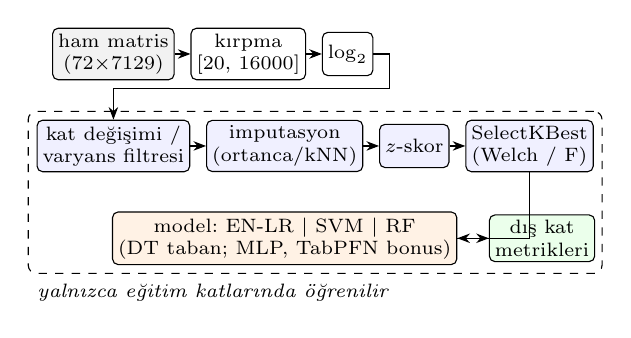
\begin{tikzpicture}[node distance=2.6mm and 2mm,
  box/.style={draw, rounded corners=2pt, align=center, font=\scriptsize, minimum height=5.5mm, inner sep=2pt, fill=white},
  fold/.style={draw, dashed, rounded corners=3pt, inner sep=3pt},
  >={Stealth[length=1.6mm]}]
\node[box, fill=gray!10] (raw) {ham matris\\(72$\times$7129)};
\node[box, right=of raw] (clip) {kırpma\\{[20, 16000]}};
\node[box, right=of clip] (log) {$\log_2$};
\node[box, below=5mm of raw, fill=blue!6] (filt) {kat değişimi /\\varyans filtresi};
\node[box, right=of filt, fill=blue!6] (imp) {imputasyon\\(ortanca/kNN)};
\node[box, right=of imp, fill=blue!6] (z) {$z$-skor};
\node[box, right=of z, fill=blue!6] (kb) {SelectKBest\\(Welch / F)};
\node[box, below=5mm of imp, fill=orange!10, minimum width=34mm] (model) {model: EN-LR $|$ SVM $|$ RF\\(DT taban; MLP, TabPFN bonus)};
\node[box, right=4mm of model, fill=green!8] (eval) {dış kat\\metrikleri};
\draw[->] (raw) -- (clip); \draw[->] (clip) -- (log);
\draw[->] (log.east) -- ++(2mm,0) |- ([yshift=4mm]filt.north) -- (filt.north);
\draw[->] (filt) -- (imp); \draw[->] (imp) -- (z); \draw[->] (z) -- (kb);
\draw[->] (kb.south) |- (model.east);
\draw[->] (model) -- (eval);
\begin{scope}[on background layer]
\node[fold, fit=(filt)(kb)(model), label={[font=\scriptsize\itshape, anchor=north west]south west:yalnızca eğitim katlarında öğrenilir}] {};
\end{scope}
\end{tikzpicture}
\caption{Planlanan sızıntısız işlem hattı. Durumsuz adımlar (kırpma, $\log_2$) bölmeden önce gelebilir; veriden öğrenen her adım (kesikli kutu), her iç ve dış eğitim katında yeniden öğrenilen bir \texttt{sklearn} \texttt{Pipeline} aşamasıdır.}
\label{fig:pipeline}
\end{figure}

\section{Ek EDA şekilleri}\label{app:figs}
\begin{figure}[!h]
\centering
\fig[width=0.95\textwidth]{fig_golub_batch.pdf}
\caption{Golub eğitim ve bağımsız set. (a) Present çağrı oranı ve (b) bölme ve sınıfa göre dizi parlaklığı. (c) Her sınıf içinde eğitim ve testi karşılaştıran gen bazlı KS $p$ değerleri; ALL'de 0 yakınındaki fazlalık dağılım kaymasına işaret eder.}
\label{fig:batch}
\end{figure}
\begin{table}[!h]
\caption{Her kohortta Welch $p$ değerine göre ilk 12 gen ($\Delta$: kohortun log ölçeğinde AML$-$ALL ortalama farkı; $t>0$: AML'de yüksek).}
\label{tab:genes}
\centering\scriptsize\setlength{\tabcolsep}{1.6pt}
\begin{tabular}{@{}r lrr lrr lrr@{}}
\toprule
 & \multicolumn{3}{c}{Golub} & \multicolumn{3}{c}{MILE} & \multicolumn{3}{c}{Andersson}\\
\cmidrule(lr){2-4}\cmidrule(lr){5-7}\cmidrule(l){8-10}
\# & gen & $\Delta$ & $t$ & gen & $\Delta$ & $t$ & gen & $\Delta$ & $t$\\ \midrule
1 & MGST1 & +4{,}10 & +13{,}5 & PNKD & +0{,}25 & +56{,}8 & PILRB & \ensuremath{-}2{,}95 & \ensuremath{-}16{,}0\\
2 & CST3 & +5{,}82 & +12{,}4 & LEF1-AS1 & \ensuremath{-}0{,}35 & \ensuremath{-}59{,}5 & INOC1 & \ensuremath{-}1{,}61 & \ensuremath{-}15{,}0\\
3 & TCF3 & \ensuremath{-}2{,}07 & \ensuremath{-}11{,}8 & LEF1 & \ensuremath{-}0{,}31 & \ensuremath{-}52{,}5 & NPY & \ensuremath{-}5{,}62 & \ensuremath{-}15{,}1\\
4 & ZYX & +3{,}83 & +11{,}0 & CFD & +0{,}43 & +49{,}8 & -- & -- & --\\
5 & CD33 & +2{,}26 & +11{,}3 & APLP2 & +0{,}21 & +49{,}3 & NPR1 & \ensuremath{-}3{,}31 & \ensuremath{-}14{,}4\\
6 & APLP2 & +2{,}77 & +9{,}6 & LOC101928615 & +0{,}22 & +48{,}8 & PCBD1 & +2{,}98 & +15{,}9\\
7 & CD79B & \ensuremath{-}4{,}45 & \ensuremath{-}9{,}2 & MGST1 & +0{,}38 & +53{,}2 & C17orf58 & +2{,}11 & +16{,}7\\
8 & POU2AF1 & \ensuremath{-}3{,}09 & \ensuremath{-}9{,}6 & MGST1 & +0{,}41 & +50{,}7 & SPG20 & +3{,}07 & +13{,}9\\
9 & DNTT & \ensuremath{-}4{,}44 & \ensuremath{-}9{,}4 & LEF1 & \ensuremath{-}0{,}37 & \ensuremath{-}55{,}1 & LOC201229 & \ensuremath{-}3{,}50 & \ensuremath{-}14{,}7\\
10 & CCND3 & \ensuremath{-}2{,}06 & \ensuremath{-}9{,}2 & CTSA & +0{,}20 & +48{,}2 & CTSC & +2{,}38 & +14{,}8\\
11 & VPREB1 & \ensuremath{-}4{,}24 & \ensuremath{-}8{,}6 & FUCA2 & +0{,}24 & +47{,}9 & PCBD1 & +2{,}99 & +14{,}6\\
12 & RHOG & +3{,}17 & +8{,}6 & LEF1-AS1 & \ensuremath{-}0{,}25 & \ensuremath{-}47{,}3 & CD33 & +3{,}87 & +17{,}7\\
\bottomrule
\end{tabular}

\end{table}
\begin{figure}[!h]
\centering
\fig[width=0.95\textwidth]{fig_class_distribution.pdf}
\caption{Sınıf dağılımı. (a) Golub referans bölmesi; (b) 14 ALL/AML alt sınıfının iki etikete eşlenmesinden sonra MILE; (c) normal kontroller çıkarıldıktan sonra Andersson. Tüm setler ALL yönünde dengesizdir.}
\label{fig:classes}
\end{figure}
\begin{figure}[!h]
\centering
\fig[width=0.95\textwidth]{fig_golub_log_distributions.pdf}
\caption{Dizi başına Golub yoğunlukları: (a) kırpma ve $\log_2$ öncesi, (b) sonrası (renk: referans bölme). (c) Gen standart sapması ve ortalaması: doğrusal ölçekte SS ortalamayla büyür ($\rho=\GolubRhoLin$), $\log_2$ sonrası bağımlılık büyük ölçüde kaybolur ($\rho=\GolubRhoLog$).}
\label{fig:logdist}
\end{figure}
\begin{figure}[!h]
\centering
\fig[width=0.95\textwidth]{fig_golub_embedding.pdf}
\caption{Golub: PCA varyans grafiği (çubuk: bileşen başına, çizgi: kümülatif), PCA ve t-SNE. PC1 \%\GolubPCOne{}, on PC \%\GolubCumTen{} açıklar; \%80 için \GolubNEighty{} PC gerekir. Varyans çok sayıda yöne yayılmıştır, yine de PC1 tek başına sınıfları ayırır.}
\end{figure}
\begin{figure}[!h]
\centering
\fig[width=0.95\textwidth]{fig_golub_volcano.pdf}
\caption{Golub: (a) Welch testlerinin volkan grafiği (renk: BH $q<0{,}05$): \GolubUpAML{} gen AML'de, \GolubUpALL{} gen ALL'de yüksektir; yani farklar tek yönlü değildir. (b) Golub'un sinyal-gürültü oranı ile Welch $t$ genleri neredeyse aynı sıralar ($\rho=\GolubRhoSNR$); tek değişkenli filtrede aralarındaki seçim önemsizdir.}
\end{figure}
\begin{figure}[!h]
\centering
\fig[width=0.95\textwidth]{fig_mile_samples.pdf}
\caption{MILE: (a) aralık ölçekli log değerlerinin dizi başına kantilleri (ortancaya göre sıralı). Kantil normalizasyonundan beklendiği gibi tüm dizilerin kantilleri aynıdır, dizi düzeyinde aykırı değer yoktur. (b) Prob seti başına eksik değer: \MileAllMissing{} prob seti tüm dizilerde boştur (çıkarıldı); diğerleri tamdır.}
\label{fig:mile_samples}
\end{figure}
\begin{figure}[!h]
\centering
\fig[width=0.95\textwidth]{fig_mile_embedding.pdf}
\caption{MILE: PCA varyans grafiği, PCA ve t-SNE (en değişken 5.000 prob). PC1 \%\MilePCOne{} açıklar ve ALL'yi AML'den ayırır (AUC \MileBestPCAUC); t-SNE'de ALL örnekleri, MILE'daki çok sayıda ALL alt tipiyle uyumlu olarak birkaç alt küme oluşturur.}
\end{figure}
\begin{figure}[!h]
\centering
\fig[width=0.95\textwidth]{fig_mile_volcano.pdf}
\caption{MILE: (a) volkan grafiği; $x$ ekseni aralık ölçekli log değerlerinin farkıdır, $p<10^{-300}$ değerleri 300'de çizilmiştir. $n=\MileN$ ile prob setlerinin \%\MileSigPct'i $q<0{,}05$ düzeyine ulaşır; bu nedenle gen seçiminde $p$ değil etki büyüklüğü yol göstermelidir. (b) SNR--$t$ uyumu.}
\end{figure}
\begin{figure}[!h]
\centering
\fig[width=0.95\textwidth,height=0.6\textheight,keepaspectratio]{fig_mile_heatmap.pdf}
\caption{MILE: ilk 30 genin kümelenmiş ısı haritası. En üst düzeydeki iki küme ALL/AML ile örtüşür (ARI \MileARI); ALL içinde bir alt küme B hücre genlerinden (EBF1, CD79A, BLK, POU2AF1) yoksundur, bu T-ALL ile tutarlıdır.}
\end{figure}
\begin{figure}[!h]
\centering
\fig[width=0.95\textwidth]{fig_andersson_samples.pdf}
\caption{Andersson: (a) dizi başına $\log_2$ oran dağılımları, lowess normalizasyonu ve merkezlemeden beklendiği gibi 0 yakınında ve benzer yayılımdadır; (b) raportör başına eksik değer: \AndGenesMissing{} raportörde boşluk vardır, \AndGenesMissingTwenty{} raportörde \%20'den fazlası eksiktir; bu nedenle (kat içi) imputasyon gereklidir.}
\label{fig:and_samples}
\end{figure}
\begin{figure}[!h]
\centering
\fig[width=0.95\textwidth]{fig_andersson_embedding.pdf}
\caption{Andersson: PCA varyans grafiği, PCA ve t-SNE (yalnızca görselleştirme için ortanca imputasyonu). PC1 \%\AndPCOne{} açıklar ve AML ile ALL'yi neredeyse kusursuz sıralar (AUC \AndPCOneAUC); t-SNE ayrı bir AML grubu ve birkaç ALL alt grubu gösterir.}
\end{figure}
\begin{figure}[!h]
\centering
\fig[width=0.95\textwidth]{fig_andersson_volcano.pdf}
\caption{Andersson: (a) volkan grafiği ($x$: $\log_2$ oranlarının farkı); raportörlerin \%\AndSigPct'si $q<0{,}05$ düzeyine ulaşır ve AML'de yüksek (\AndUpAML) ile ALL'de yüksek (\AndUpALL) olarak eşit bölünür. (b) SNR--$t$ uyumu.}
\end{figure}
\begin{figure}[!h]
\centering
\fig[width=0.95\textwidth,height=0.6\textheight,keepaspectratio]{fig_andersson_heatmap.pdf}
\caption{Andersson: ilk 30 genin kümelenmiş ısı haritası. Soy çubuğu: açık mavi B soylu ALL, koyu mavi T hücreli ALL, turuncu AML. T-ALL örnekleri AML'nin yanında kümelenir.}
\end{figure}

\end{document}
